% -*- coding: utf-8 -*-
\newpage
\section{Computational Framework}

In this section, we describe the computational protocols and methodologies
adopted in this study.  All bespoke software was developed for Unix-like
environments and has been validated under both \textsc{GNU}-\Linux and \macOS.
% No attempt has been made, nor will be made, to support Microsoft Windows.

\subsection{Amsterdam Modeling Suite}\label{ams_section}

The majority of quantum chemical computations were performed using the
Amsterdam Modeling Suite (\ams), a commercial software package developed by the
Software for Chemistry and Materials (\scm) company~\cite{ams2025}. Originally
developed in the 70's within the theoretical chemistry department of the Vrije
Universiteit in Amsterdam, \ams has evolved from its early \fortran foundations
to include a broad set of modern features. These include support for
Object-Oriented Programming (OOP), modular design, and an expanding set of
functionalities via successive versions.

Some engines in \ams such as \adf, \band, and \dftb remain written in modern
\fortran. While the graphical user interface (\gui) is based on \tcl,
several high-performance modules have been implemented in C++. A
significant extension is the \python based scripting interface \plams (Python
Library for Automating Molecular Simulations), which provides high-level access
to workflow automation, job management, and data analysis across \ams engines.

\begin{figure}[h!]
  \centering
  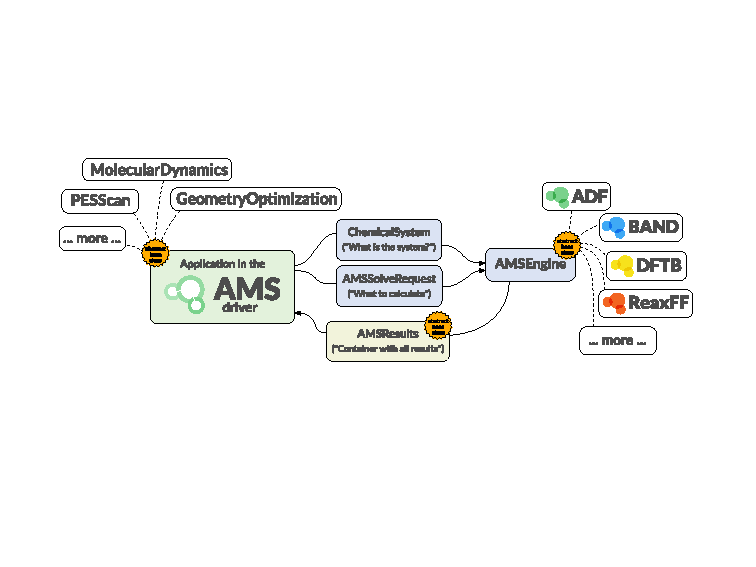
\includegraphics[width=1\textwidth]{img/ams_driver}
  \caption{The AMS driver and its interaction with available engines. Diagram
           taken from the developer meeting slides of \scm, 2025.}
  \label{ams_engines}
\end{figure}

\newpage
In this work, we primarily employed \adf, one of the most mature and
feature-rich engines within \ams. The \ams driver integrate also the QTAIM
partition in \band and \dftb.  As illustrated in Figure~\ref{ams_engines}, the
\ams driver manages the coordination of jobs, delegating tasks to the
appropriate engine according to the user-defined settings and task
requirements.

Another important tool used in this work is the \plams, which provides a
\python library not only for the \ams driver, but also with many other tools
and for sure given to the user the possibility to automatise a personal
workflow. The current development of \texttt{amspython} runs on \python 3.8 and
it can interact with libraries such as \textsc{numpy}, \textsc{scipy} or
\textsc{pandas}, (as shown in Figure~\ref{plams_diagram}) allowing the user to
perform advanced data analysis, \plams also provides functions to read binary
files created by \ams engines for direct access to molecular properties.

\begin{figure}[h]
  \centering
  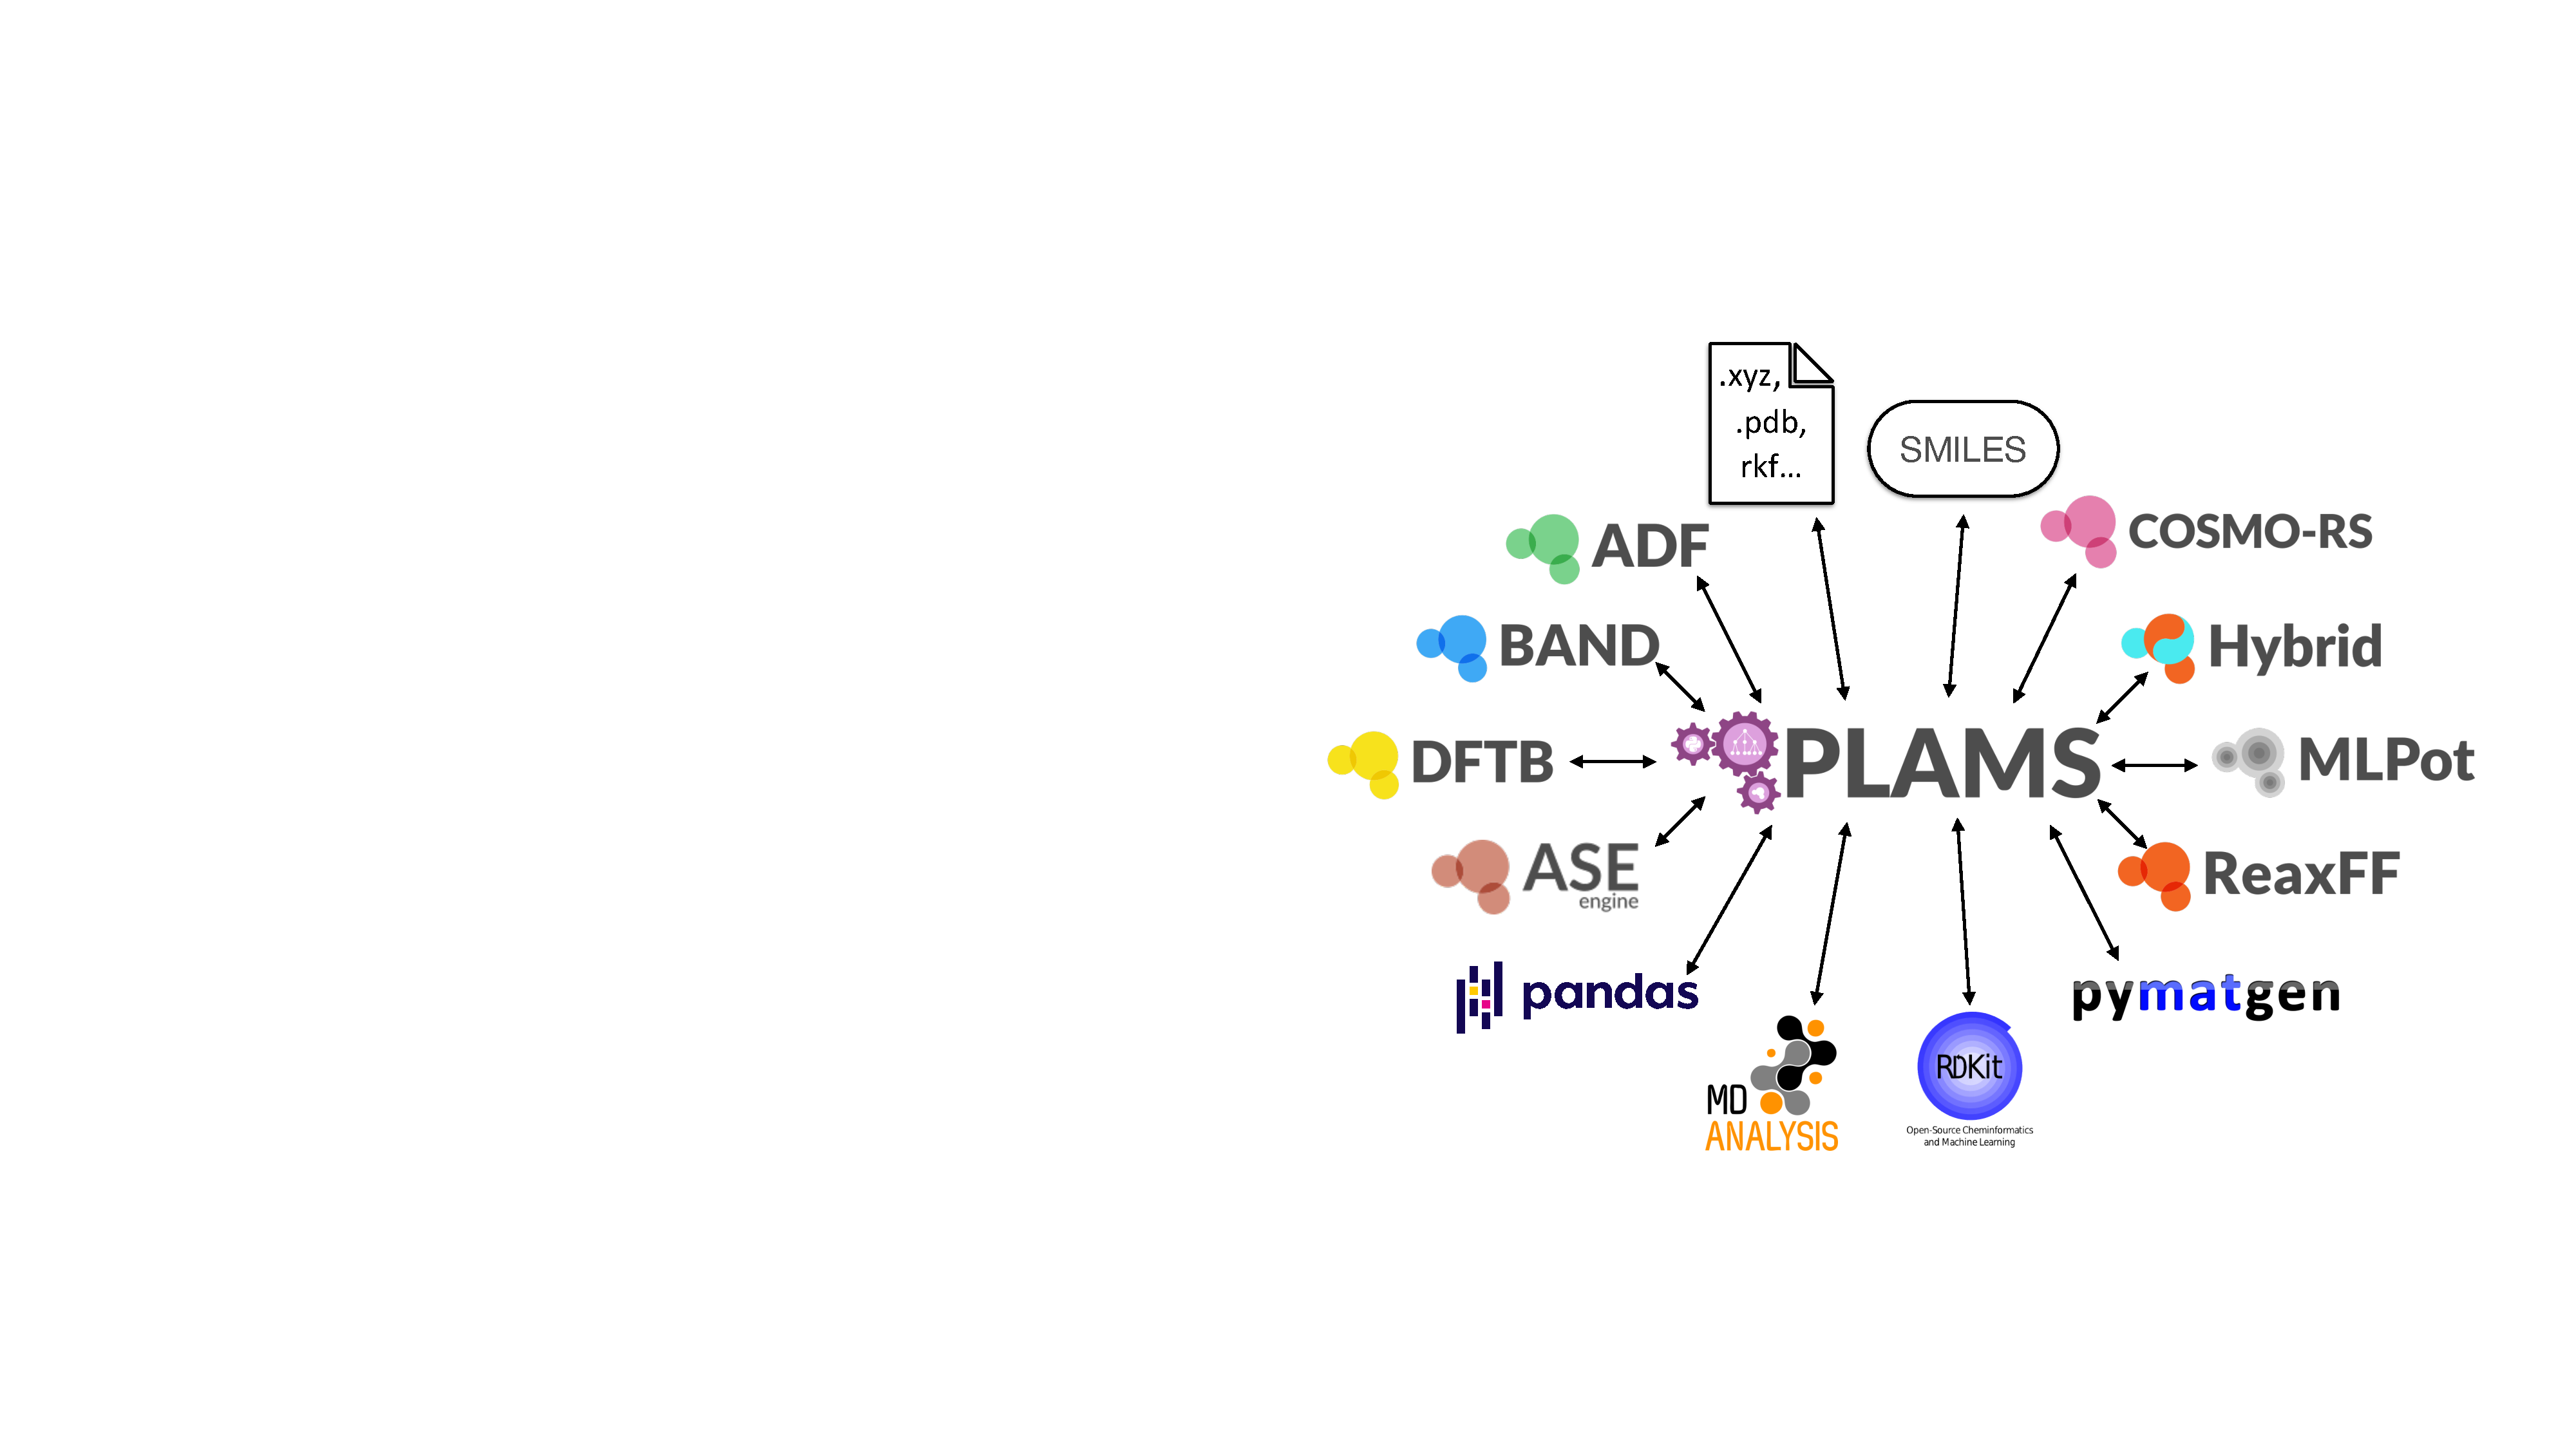
\includegraphics[width=0.75\textwidth]{img/plams_diagram}
  \caption{Interaction between \plams and different engines from \ams driver and
           other libraries. Diagram taken from the developer meeting slides of
           \scm, 2025.}
  \label{plams_diagram}
\end{figure}

While \plams is distributed as open-source software via
\href{http://www.github.com/SCM-NV/PLAMS}{\faGithub/SCM-NV/PLAMS}, the source
code of \ams is not publicly available. Access is restricted to licensed users,
and availability depends on a number of parameters including: $i$) selected
modules, $ii$) total CPU core limit, $iii$) duration of licence, and $iv$)
academic or commercial status of the institution. Source code access is
restricted to developers.

\newpage
\subsubsection{Run File Structure}

\begin{wrapfigure}{r}{0.4\textwidth}
  \centering
  \resizebox{\linewidth}{!}{% -*- coding: utf-8 -*-

% cartoon of *.run
\begin{tikzpicture}
  % Main box
  % \fontfamily{phv}\selectfont
  {\scriptsize\sffamily
  \node[rectangle, draw=strongGreen, thick,
        fill=pastelGreen, fill opacity=0.3,
        text width=5.5cm, align=left, inner sep=4pt,
        rounded corners=5pt, text=black,
        text opacity=1] (mainbox2) at (0,0) {
    \baselineskip=7pt
    \#!/bin/sh\\
    Task GeometryOptimization\\ [0.3cm]

    Properties\\
    \hspace{0.5cm}NormalModes true\\
    End\\ [0.3cm]

    System\\
    \hspace{0.5cm}Atoms\\
    \hspace{1cm} H 0.0 0.0 0.0\\
    \hspace{1cm} H 0.8 0.0 0.0\\
    \hspace{0.5cm}End\\
    End\\ [0.3cm]
    
    Engine DFTB\\
    \hspace{0.5cm}\tikz[
      baseline=(modelline.base)]{\node[rectangle,
      draw=strongBlue, fill=pastelBlue,
      fill opacity=0.7, inner sep=2pt,
      rounded corners=3pt, text=black,
      text opacity=1]
    (modelline) {Model GFN1-xTB}}\\ [-0.2cm]
    EndEngine
  };}

\end{tikzpicture}

}
  \caption{Example of an \ams run file. The blue highlighted line is the Engine
    Input, while the rest of the run file is interpreted by the \ams driver,
    independently of the chosen engine.}
  \label{ams_input}
\end{wrapfigure}

The \ams driver can be controlled via a flexible input file written in a
shell-like~\faTerminal~syntax. This run file acts not only as a traditional
input, but as a lightweight script that manages the execution of the chosen
engine. While calculations can also be launched through the \gui, scripting
provides the advantage that it enables systematic and automated workflows, such
as running multiple calculations with varying molecular geometries, basis sets,
or external fields without user intervention.

Figure~\ref{ams_input} shows the structure of a typical \ams run file. The
script defines the task (\eg single point calculation or geometry optimisation),
the properties to compute (such as normal modes), and the system under study,
which includes molecular coordinates (by default in \AA) and, optionally, a
charge or external electric field, among other settings. The \texttt{Engine}
block provides the engine-specific input and is closed with the keyword
\texttt{EndEngine}, rather than \texttt{End}.

Since the interpreter of the run file is predefined as \texttt{sh}, it can be
made executable and launched directly from the command line, like any standard
shell script. The interpreter can also be changed to match the user's preferred
shell (\eg \texttt{bash}, \texttt{zsh}, \texttt{fish}, or any other), as long
as the environment is properly set up. This setup is managed by the
\texttt{adfbashrc.sh} script, which should be sourced in the appropriate shell
initialisation file (such as \texttt{.bashrc}, \texttt{.zshrc}, etc.), ensuring
that binaries, licence information, and scratch directories are properly
configured.

Additional settings ---such as the number of processes--- can be specified
either via command-line flags or environment variables. For example, the number
of processes can be set in either of the following ways:

\newpage
\begin{lstlisting}[language=bash, numbers=none]
# 1. By a flag
"$AMSBIN/ams" -n 1 << eor
    # ams input
eor
# 2. By an environment variable
export NSCM=1
"$AMSBIN/ams" << eor
    # ams input
eor
\end{lstlisting}

A general procedure for executing a calculation with the \ams driver
---independent of the engine used--- is illustrated below. The user writes a
run file, makes it executable, and launches it from the command line. Upon
execution, a new directory named \texttt{``\$\{AMS\_JOBNAME\}.results''} is
automatically created to store auxiliary files:

\lstset{style=terminal, numbers=none, escapeinside={(*@}{@*)}}
\begin{macterminal}[vcastor@ada - bash]
$ # Create a run file
$ vi run_file.run             # or any preferred text editor
$ chmod u+x run_file.run      # Make it executable
$ ./run_file.run ~ output.out # Execute and redirect output
$ # A new directory named ${AMS_JOBNAME}.results will be created
\end{macterminal}
\lstset{style=mystyle}

The resulting \texttt{*.results} directory contains a log file and two
\texttt{*.rkf} files ---one generated by the \ams driver and the other by the
selected engine---. In addition, the directory may include several auxiliary
files such as \texttt{TAPE10}, \texttt{TAPE13}, \texttt{TAPE15}, and
\texttt{TAPE41}, as well as a separate \texttt{TAPE21} file for each element
present in the system, and sometimes the binary \texttt{t12.rel} file, which is
not a KF file, but an auxiliary file specific to relativistic calculations.
Depending on the nature of the task binary scratch files may be created. If no
job name is provided, the default name \texttt{ams.results} is used. The
\texttt{*.rkf} files are binary containers developed by \ams to store
structured information from the calculation. Human-readable output is printed
directly to \texttt{stdout} and \texttt{stderr} during execution.

\newpage

\begin{wrapfigure}{r}{0.65\textwidth}
  \centering
  % \vspace{-0.4cm}%
  \resizebox{\linewidth}{!}{% -*- coding: utf-8 -*-

\begin{tikzpicture}[
  dirtree,
  % Even less indentation
  level 1/.style={sibling distance=0.7cm, level distance=1.5cm},
  level 2/.style={sibling distance=0.7cm, level distance=1.3cm},
  level 3/.style={sibling distance=0.7cm, level distance=1.1cm},
]

  \node[directory] (root) {work\_dir/}
    child { node[file] (run) {azulene.run} }
    child { node[file] (out) {azulene.out} }
    child { node[directory] (results) {results/}
      child { node[file] (log) {ams.log} }
      child { node[file] (amsrkf) {ams.rkf} }
      child { node[file] (adfrkf) {adf.rkf} }
      child { node[file] (create) {CreateAtoms.out} }
      child { node[file] (t21H) {t21.\emph{number}.H} }
      child { node[file] (dots1) {...} }
      child { node[file] (t21C) {t21.\emph{number}.C} }
    };

  % Add all comments aligned at x=6.5
  \node[comment] at (6.5,0 |- root) {directory where the calculation ran};
  \node[comment] at (6.5,0 |- run) {run script};
  \node[comment] at (6.5,0 |- out) {human readable output};
  \node[comment] at (6.5,0 |- log) {log file from the \ams driver};
  \node[comment] at (6.5,0 |- amsrkf) {binary file of the \ams driver};
  \node[comment] at (6.5,0 |- adfrkf) {binary file of the \adf engine};
  \node[comment] at (6.5,0 |- create) {summary by atom type};
  \node[comment] at (6.5,0 |- t21H) {TAPE21 for H atoms};
  \node[comment] at (6.5,0 |- dots1) {TAPE21 for every atom type};
  \node[comment] at (6.5,0 |- t21C) {TAPE21 for C atoms};

\end{tikzpicture}
}
  \caption{work directory structure for a Single Point Calculation with
    the \adf engine.} 
  \label{ams_dir_structure}
\end{wrapfigure}

Figure~\ref{ams_dir_structure} illustrates the file structure within the
\texttt{*.results} directory for a single point calculation. In the case of a
geometry optimisation, the directory will additionally contain an
\texttt{.rkf} file for each optimisation step, named
\texttt{GOStep}\textit{n}\texttt{.rkf}, where \textit{n} corresponds to the step
number.

The following two examples demonstrate how a run script can be used to automate
calculations by looping over different molecular geometries or computational
settings. The first example illustrates how to set up a geometry scan
using a scripted approach.

\begin{lstlisting}[language=bash]
#!/bin/bash

# Edge lengths for each system
edge_lengths=(2.700 2.200 2.150 2.120 2.090 2.070 1.960 1.800)

# Function to calculate coordinates
calculate_x() {
  local length=$1
  echo "scale=6; $length/2" | bc -l
}
calculate_y() {
  local length=$1
  echo "scale=6; $length*sqrt(3)/2" | bc -l
}

# Loop to generate AMS input files and run calculations
for i in "${!edge_lengths[@]}"; do
  length="${edge_lengths[$i]}"
  y_coord=$(calculate_y "$length")
  x_coord=$(calculate_x "$length")

  # Variable with the job name; and execute the AMS driver [binary]
  AMS_JOBNAME="be_${i}" $AMSBIN/ams << eor

Task SinglePoint
System
  Atoms
    Be 0.000000 0.000000 0.000000
    Be $length 0.000000 0.000000
    Be $x_coord $y_coord 0.000000
  End
  Charge -2
End

Engine ADF
  # Engine specific input
EndEngine

eor

done
\end{lstlisting}

The same principle can be extended to alter not only molecular coordinates, but
also keywords such as the basis set, external fields, numerical
settings, or solvation models. This flexibility enables fully reproducible and
automated protocols.

\begin{lstlisting}[language=bash]
#!/bin/bash
# This ADF input has a loop to compute a system with an external electric field
# in different directions
# x, y, z, -x, -y and -z [V/Å]  (0.0100 a. u.)

declare -A EFvalues
nrows=7
ncolumns=3
name=( x y z mx my mz noE )

for ((i=0; i<nrows; i++)) do
  for ((j=0; j<ncolumns; j++)) do
    EFvalues[$i,$j]=0.00
    k=$(expr $i - 3)
    if [ $i -eq $j ]; then
      EFvalues[$i,$j]=0.5144
    elif [ $j -eq $k ]; then
      EFvalues[$i,$j]=-0.5144
    fi
  done
done

for ((j=0;j<nrows;j++)) do

AMS_JOBNAME=system_${name[$j]} $AMSBIN/ams << eor

Task SinglePoint
System
  Atoms
    O     -0.9952892833      1.0793836907     -0.8870331216
    C      0.3806786652      0.8563670307     -0.5242410141
    C      1.1343132702      2.1207737537     -1.0892343026
    # Molecular coordinates
  End
  ElectrostaticEmbedding
    ElectricField ${EFvalues[$j,0]} ${EFvalues[$j,1]} ${EFvalues[$j,2]}
  End
End

Engine ADF
  # Engine specific input
EndEngine

eor

done
\end{lstlisting}

It is important to note that when a calculation is launched from the \gui, the
\texttt{TAPE10} file is automatically saved. In contrast, when using a run file,
\texttt{TAPE10} must be explicitly requested within the Engine block;
otherwise, it will not be retained after the calculation finishes. Although
\texttt{TAPE10} primarily contains temporary data, it is required for certain
types of analysis within the \gui ---for instance, the visualisation of atomic
basins in the QTAIM partition.

\begin{wrapfigure}[7]{l}{0.4\textwidth}
  \centering
  \vspace{1.4cm}%
  
\includegraphics[width=0.4\textwidth]{img/tutorial_logo.png}
\end{wrapfigure}

Additional options can be specified directly in the input file, such as
disabling molecular symmetry or adjusting numerical quality thresholds. For
further information, users are encouraged to consult the official \ams
documentation and tutorials, available at:
\href{http://www.scm.com/doc/Documentation/}{scm.com/doc/Documentation} and
\href{http://www.scm.com/doc/Tutorials/}{scm.com/doc/Tutorials}.

\newpage
\subsection{Numerical Stability}

As with any numerical approach, it is essential to remain aware of
finite-precision effects. A well-known example is the inexactness of
floating-point arithmetic (\eg $0.1 + 0.2 \neq 0.3$), which arises from the
limitations of binary representation as defined by the IEEE 754 standard. While
such discrepancies are typically small ---on the order of $10^{-17}$--- and
often negligible in practical workflows, they are not confined to artificial
examples.  Even robust, low-level numerical libraries such as
\lapack~\cite{laug} can exhibit numerical instability in certain contexts.

\begin{table}[h]
  \centering
  \caption{Floating-point representation of $0.1$, $0.2$, and $0.3$ in IEEE 754
    single precision format.}
  % \color{terminalgreen!80!terminalblack}
  \rowcolors{1}{backcolour}{backcolour}
  \ttfamily
  \begin{tabular}{l|c|c|l}
  Decimal     & Sign & Exponent (bias) & Mantissa (binary) \\
  \hline
  0.1         & 0    & 01111011 (123)  & 10011001100110011001101 \\
  0.2         & 0    & 01111100 (124)  & 10011001100110011001101 \\
  \hline
  0.1 + 0.2   & 0    & 01111101 (125)  & 00110011001100110011010 \\
  0.3         & 0    & 01111101 (125)  & 00110011001100110011001 \\
  \end{tabular}
  \label{ieee754_fp}
\end{table}

Dhillon~\cite{Dhillon1998} has shown that inverse iteration algorithms, as
implemented in \lapack, can fail to compute eigenvectors accurately
when eigenvalues are nearly degenerate. This is primarily due to breakdowns in
reorthogonalisation and heightened sensitivity to small perturbations. Demmel et
al.~\cite{Demmel2008} further explored the numerical stability of eigenvalue
solvers, observing that Bisection/Inverse Iteration (BI) schemes, including
\subroutines such as \texttt{DGELSS}, may lose orthogonality when eigenvalues are
clustered.

To mitigate such issues, it is good practice to incorporate validation
procedures and redundancy checks, especially for tasks involving eigenvalue
problems with closely spaced spectra.

It should be emphasised, however, that such numerical instabilities are
edge cases and are rarely encountered in routine applications. For the majority
of computational tasks carried out in this work, the numerical precision
provided by the \fortran-based implementations and the \lapack library proved
entirely sufficient.

\newpage
\subsection{Code Management}

\begin{wrapfigure}{r}{0.3\textwidth}
  \centering
  
\includegraphics[width=0.27\textwidth]{img/Gitea_Logo.pdf}
\end{wrapfigure}

All software, scripts, and data files used in this project were managed using
version control systems, primarily \git and \textsc{svn}. Several contributions
developed during this work have been integrated into the main (trunk)
development branch~\faCodeBranch\xspace of \ams, while others remain in feature
branches awaiting final integration. In 2024, \scm transitioned from
\textsc{svn} to Gitea, a web-based platform for managing \git repositories.

Supplementary scripts~\faCode\xspace and workflows are publicly available at
\href{http://www.github.com/vcastor/PhDscripts}{\faGithub/vcastor/PhDScripts}.
The complete manuscript, including code, figures, and additional material, is
archived at:
\href{http://www.github.com/vcastor/PhDManuscript}{\faGithub/vcastor/PhDManuscript}.
Details on compilation, execution, and reproduction of the manuscript are
provided in Appendix~\ref{how_written}.

\scriptsize
\begin{flushright}
  \textit{For further technical queries,\\
  please contact the author directly.}
\end{flushright}
\normalsize

